\section{C++ Quick Start}

\subsection{C++ vs C: Key Differences}

% 本页展示 C++ 的所有运算符
\begin{frame}[fragile]{C++ Operators and Keywords (From \textcolor{blue}{\href{https://en.cppreference.com/w/cpp/language/}{cppreference.com}})}
    \begin{columns}
        \begin{column}{0.6\textwidth}
    \begin{figure}
        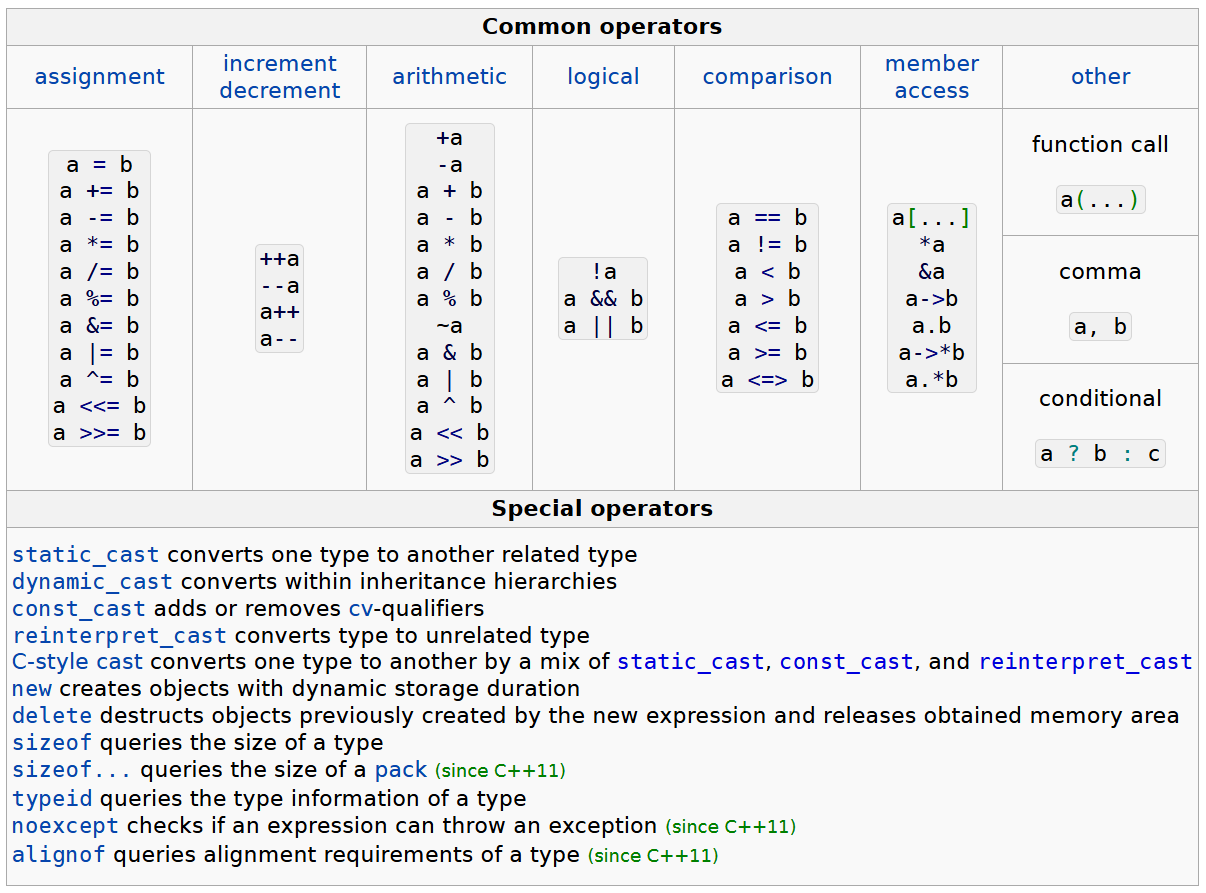
\includegraphics[width=\textwidth]{day8_pm/img/1-operators}
    \end{figure}
        \end{column}
        \begin{column}{0.4\textwidth}
            \begin{figure}
                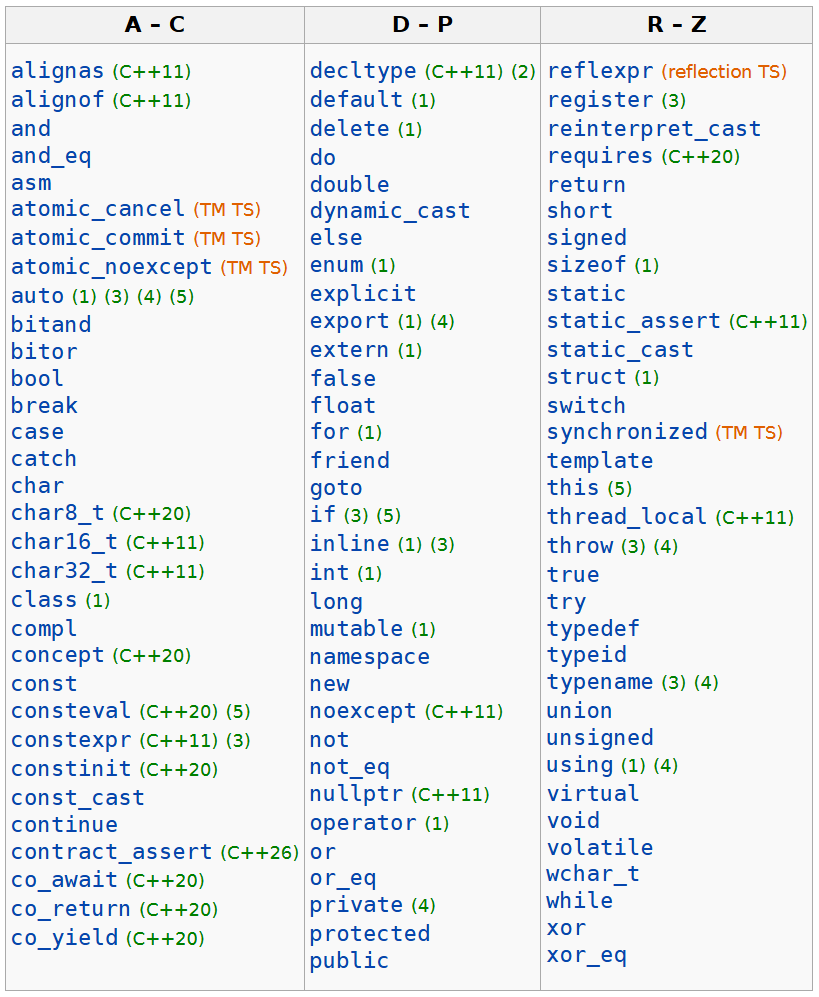
\includegraphics[width=0.9\textwidth]{day8_pm/img/1-keywords}
            \end{figure}
        \end{column}
    \end{columns}
\end{frame}

\begin{frame}[fragile]{\emoji{gear} C++ Operators and Keywords}
    We'll meet some new friends in this class:
    \begin{itemize}
        \item \textbf{I/O}:  \texttt{>>}, \texttt{<<}
        \item \textbf{Memory}: \texttt{new}, \texttt{delete}, \texttt{new[]}, \texttt{delete[]}
        \item \textbf{Type System}: \texttt{auto}, \texttt{decltype}, \texttt{using}
        \item \textbf{Class}: \texttt{::}, \texttt{public}, \texttt{private}, \texttt{protected}, \texttt{friend}, \texttt{virtual}, \texttt{override}, \texttt{final}
    \end{itemize}
\end{frame}
    
\begin{frame}[fragile]{\emoji{gear} C Standard I/O vs I/O Streams}
	\begin{columns}
		\begin{column}{0.5\textwidth}
			\textbf{C Style}
			\begin{minted}{c}
#include <stdio.h>
#include <stdlib.h>

void print_msg(void) {
    printf("Hello from C!\n");
}

int main() {
    FILE* fp = fopen("test.txt", "r");
    if (fp) {
        // Manual resource management
        char line[100];
        while (fgets(line, 100, fp) != NULL) {
            printf("%s", line);
        }
        fclose(fp);
    }
    return 0;
}
			\end{minted}
		\end{column}
		\begin{column}{0.5\textwidth}
			\textbf{C++ Style}
			\begin{minted}{cpp}
#include <iostream>
#include <fstream>

void print_msg() {
    std::cout << "Hello from C++!" << std::endl;
}

int main() {
    std::ifstream file("test.txt");
    if (file.is_open()) {
        // Automatic resource management
        std::string line;
        while (std::getline(file, line)) {
            std::cout << line << std::endl;
        }
    }
    return 0;
}
			\end{minted}
		\end{column}
	\end{columns}
\end{frame}

% 上页给出代码对比,本页给出讲解
\begin{frame}[fragile]{\emoji{gear} C Standard I/O vs I/O Streams}
    \begin{itemize}
        \item \textbf{C Standard I/O}:
            \begin{itemize}
                \item Uses functions like \texttt{printf}, \texttt{fopen}, and \texttt{fclose}
                \item Requires manual resource management
            \end{itemize}
        \item \textbf{C++ I/O Streams}:
            \begin{itemize}
                \item Uses classes like \texttt{std::cout}, \texttt{std::ifstream}, and \texttt{std::ofstream}
                \item Automatically manages resources
                \item \textbf{Stream Operators}: \texttt{<<} and \texttt{>>}
            \end{itemize}
    \end{itemize}
    \vspace{0.5em}
    \textbf{Benefits of C++ Streams:}
    \begin{itemize}
        \item Type safety and flexibility
        \item Easier to read and maintain code
        \item Automatic resource cleanup when objects go out of scope
    \end{itemize}
\end{frame}

% 介绍命名空间,标准库的所有名字都在命名空间 std 中;并介绍 << >> 运算符
\begin{frame}[fragile]{\emoji{gear} C Standard I/O vs I/O Streams}
    \begin{itemize}
        \item \textbf{Namespaces}:
            \begin{itemize}
                \item C++ uses namespaces to avoid name collisions
                \item Standard library functions and classes are in the \texttt{std} namespace
            \end{itemize}
        \item \textbf{Stream Operators}:
            \begin{itemize}
                \item \texttt{<<} is used for output (stream insertion)
                \item \texttt{>>} is used for input (stream extraction)
            \end{itemize}
    \end{itemize}
    \vspace{0.5em}
    \textbf{Example:}
    \begin{minted}{cpp}
std::cout << "Hello, World!" << std::endl;
std::cin >> user_input;
    \end{minted}
\end{frame}


\begin{frame}[fragile]{\emoji{link} References vs Pointers}
	\begin{columns}
		\begin{column}{0.5\textwidth}
			\textbf{C Pointers}
			\begin{minted}{c}
void swap_c(int* a, int* b) {
    int temp = *a;
    *a = *b;
    *b = temp;
}
int main() {
    int x = 5, y = 10;
    swap_c(&x, &y);  // Pass addresses
    printf("x=%d, y=%d\n", x, y);
    return 0;
}
			\end{minted}
		\end{column}
		\begin{column}{0.5\textwidth}
			\textbf{C++ References}
			\begin{minted}{cpp}
void swap_cpp(int& a, int& b) {
    int temp = a;
    a = b;
    b = temp;
}
int main() {
    int x = 5, y = 10;
    swap_cpp(x, y);  // Direct pass
    std::cout << "x=" << x << ", y=" << y << std::endl;
    return 0;
}
			\end{minted}
		\end{column}
	\end{columns}

	\vspace{0.5em}
	\begin{itemize}
		\item References must be initialized and cannot be reassigned
		\item Cleaner syntax for function parameters
	\end{itemize}
\end{frame}

\subsection{Essential Features for Concurrency}
\begin{frame}[fragile]{\emoji{rocket} Lambda Expressions: The Core of Thread Functions}
	\begin{columns}
		\begin{column}{0.5\textwidth}
			\textbf{C Function Pointers}
			\begin{minted}{c}
#include <pthread.h>

void* thread_func(void* arg) {
    int id = *(int*)arg;
    printf("Thread %d running\n", id);
    return NULL;
}

int main() {
    pthread_t thread;
    int id = 1;
    pthread_create(&thread, NULL,
                   thread_func, &id);
    pthread_join(thread, NULL);
    return 0;
}
			\end{minted}
		\end{column}
		\begin{column}{0.5\textwidth}
			\textbf{C++ Lambda}
			\begin{minted}{cpp}
#include <thread>
#include <iostream>

int main() {
    int id = 1;

    // Lambda expression
    auto thread_func = [id]() {
        std::cout << "Thread " << id
                  << " running" << std::endl;
    };

    std::thread t(thread_func);
    t.join();

    return 0;
}
			\end{minted}
		\end{column}
	\end{columns}

	\vspace{0.5em}
	\textbf{Lambda Capture Modes:}
	\begin{itemize}
		\item \texttt{[]} - Capture nothing
		\item \texttt{[=]} - Capture by value
		\item \texttt{[\&]} - Capture by reference
		\item \texttt{[id]} - Capture specific variable by value
	\end{itemize}
\end{frame}

\begin{frame}[fragile]{\emoji{brain} Auto Type Deduction \& Smart Pointers}
	\begin{columns}
		\begin{column}{0.5\textwidth}
			\textbf{Auto Type Deduction}
			\begin{minted}{cpp}
#include <vector>
#include <map>

int main() {
    auto x = 42;              // int
    auto y = 3.14;            // double
    auto str = "Hello";       // const char*

    std::vector<int> vec{1,2,3};
    auto it = vec.begin();    // vector<int>::iterator

    // Complex types made simple
    std::map<std::string, int> m;
    for(auto& pair : m) {     // Range-based for
        std::cout << pair.first << std::endl;
    }

    return 0;
}
			\end{minted}
		\end{column}
		\begin{column}{0.5\textwidth}
			\textbf{Smart Pointers}
			\begin{minted}{cpp}
#include <memory>

class Resource {
public:
    Resource() { std::cout << "Created\n"; }
    ~Resource() { std::cout << "Destroyed\n"; }
};

int main() {
    // Automatic memory management
    auto ptr = std::make_unique<Resource>();

    // Shared ownership
    auto shared1 = std::make_shared<Resource>();
    auto shared2 = shared1;  // Reference count: 2

    // Automatic cleanup when out of scope
    return 0;
}
			\end{minted}
		\end{column}
	\end{columns}

	\vspace{0.5em}
	\textbf{Benefits:}
	\begin{itemize}
		\item Automatic memory management
		\item Exception safety
		\item Clear ownership semantics
	\end{itemize}
\end{frame}
